% UCL Thesis LaTeX Template
%  (c) Ian Kirker, 2014
% 
% This is a template/skeleton for PhD/MPhil/MRes theses.
%
% It uses a rather split-up file structure because this tends to
%  work well for large, complex documents.
% We suggest using one file per chapter, but you may wish to use more
%  or fewer separate files than that.
% We've also separated out various bits of configuration into their
%  own files, to keep everything neat.
% Note that the \input command just streams in whatever file you give
%  it, while the \include command adds a page break, and does some
%  extra organisation to make compilation faster. Note that you can't
%  use \include inside an \include-d file.
% We suggest using \input for settings and configuration files that
%  you always want to use, and \include for each section of content.
% If you do that, it also means you can use the \includeonly statement
%  to only compile up the section you're currently interested in.
% You might also want to put figures into their own files to be \input.

% For more information on \input and \include, see:
%  http://tex.stackexchange.com/questions/246/when-should-i-use-input-vs-include


% Formatting rules for theses are here: 
%  http://www.ucl.ac.uk/current-students/research_degrees/thesis_formatting
% Binding and submitting guidelines are here:
%  http://www.ucl.ac.uk/current-students/research_degrees/thesis_binding_submission

% This package goes first and foremost, because it checks all 
%  your syntax for mistakes and some old-fashioned LaTeX commands.
% Note that normally you should load your documentclass before 
%  packages, because some packages change behaviour based on
%  your document settings.
% Also, for those confused by the RequirePackage here vs usepackage
%  elsewhere, usepackage cannot be used before the documentclass
%  command, while RequirePackage can. That's the only functional
%  difference as far as I'm aware.
\RequirePackage[l2tabu, orthodox]{nag}


% ------ Main document class specification ------
% The draft option here prevents images being inserted,
%  and adds chunky black bars to boxes that are exceeding 
%  the page width (to show that they are).
% The oneside option can optionally be replaced by twoside if
%  you intend to print double-sided. Note that this is
%  *specifically permitted* by the UCL thesis formatting
%  guidelines.
%
% Valid options in terms of type are:
%  phd
%  mres
%  mphil
%\documentclass[12pt,phd,draft,a4paper,oneside]{ucl_thesis}
\documentclass[12pt,phd,a4paper,oneside]{ucl_thesis}


% Package configuration:
%  LaTeX uses "packages" to add extra commands and features.
%  There are quite a few useful ones, so we've put them in a 
%   separate file.
% -------- Packages --------

% This package just gives you a quick way to dump in some sample text.
% You can remove it -- it's just here for the examples.
\usepackage{blindtext}

% This package means empty pages (pages with no text) won't get stuff
%  like chapter names at the top of the page. It's mostly cosmetic.
\usepackage{emptypage}

% The graphicx package adds the \includegraphics command,
%  which is your basic command for adding a picture.
\usepackage{graphicx}

% The float package improves LaTeX's handling of floats,
%  and also adds the option to *force* LaTeX to put the float
%  HERE, with the [H] option to the float environment.
\usepackage{float}

% The amsmath package enhances the various ways of including
%  maths, including adding the align environment for aligned
%  equations.
\usepackage{amsmath}
\usepackage{amssymb}

% Use these two packages together -- they define symbols
%  for e.g. units that you can use in both text and math mode.
% \usepackage{gensymb}
% \usepackage{textcomp}
% You may also want the units package for making little
%  fractions for unit specifications.
%\usepackage{units}


% The setspace package lets you use 1.5-sized or double line spacing.
\usepackage{setspace}
\setstretch{1.5}

% That just does body text -- if you want to expand *everything*,
%  including footnotes and tables, use this instead:
%\renewcommand{\baselinestretch}{1.5}


% PGFPlots is either a really clunky or really good way to add graphs
%  into your document, depending on your point of view.
% There's waaaaay too much information on using this to cover here,
%  so, you might want to start here:
%   http://pgfplots.sourceforge.net/
%  or here:
%   http://pgfplots.sourceforge.net/pgfplots.pdf
%\usepackage{pgfplots}
%\pgfplotsset{compat=1.3} % <- this fixed axis labels in the version I was using

% PGFPlotsTable can help you make tables a little more easily than
%  usual in LaTeX.
% If you're going to have to paste data in a lot, I'd suggest using it.
%  You might want to start with the manual, here:
%  http://pgfplots.sourceforge.net/pgfplotstable.pdf
%\usepackage{pgfplotstable}

% These settings are also recommended for using with pgfplotstable.
%\pgfplotstableset{
%	% these columns/<colname>/.style={<options>} things define a style
%	% which applies to <colname> only.
%	empty cells with={--}, % replace empty cells with '--'
%	every head row/.style={before row=\toprule,after row=\midrule},
%	every last row/.style={after row=\bottomrule}
%}


% The mhchem package provides chemistry formula typesetting commands
%  e.g. \ce{H2O}
%\usepackage[version=3]{mhchem}

% And the chemfig package gives a weird command for adding Lewis 
%  diagrams, for e.g. organic molecules
%\usepackage{chemfig}

% The linenumbers command from the lineno package adds line numbers
%  alongside your text that can be useful for discussing edits 
%  in drafts.
% Remove or comment out the command for proper versions.
%\usepackage[modulo]{lineno}
% \linenumbers 


% Alternatively, you can use the ifdraft package to let you add
%  commands that will only be used in draft versions
%\usepackage{ifdraft}

% For example, the following adds a watermark if the draft mode is on.
%\ifdraft{
%  \usepackage{draftwatermark}
%  \SetWatermarkText{\shortstack{\textsc{Draft Mode}\\ \strut \\ \strut \\ \strut}}
%  \SetWatermarkScale{0.5}
%  \SetWatermarkAngle{90}
%}


% The multirow package adds the option to make cells span 
%  rows in tables.
\usepackage{multirow}


% Subfig allows you to create figures within figures, to, for example,
%  make a single figure with 4 individually labeled and referenceable
%  sub-figures.
% It's quite fiddly to use, so check the documentation.
%\usepackage{subfig}

% The natbib package allows book-type citations commonly used in
%  longer works, and less commonly in science articles (IME).
% e.g. (Saucer et al., 1993) rather than [1]
% More details are here: http://merkel.zoneo.net/Latex/natbib.php
%\usepackage{natbib}

% The bibentry package (along with the \nobibliography* command)
%  allows putting full reference lines inline.
%  See: 
%   http://tex.stackexchange.com/questions/2905/how-can-i-list-references-from-bibtex-file-in-line-with-commentary
\usepackage{bibentry}

% The isorot package allows you to put things sideways 
%  (or indeed, at any angle) on a page.
% This can be useful for wide graphs or other figures.
%\usepackage{isorot}

% The caption package adds more options for caption formatting.
% This set-up makes hanging labels, makes the caption text smaller
%  than the body text, and makes the label bold.
% Highly recommended.
\usepackage[format=hang,font=small,labelfont=bf]{caption}

% If you're getting into defining your own commands, you might want
%  to check out the etoolbox package -- it defines a few commands
%  that can make it easier to make commands robust.
\usepackage{etoolbox}


% Sets up links within your document, for e.g. contents page entries
%  and references, and also PDF metadata.
% You should edit this!
%%
%% This file uses the hyperref package to make your thesis have metadata embedded in the PDF, 
%%  and also adds links to be able to click on references and contents page entries to go to 
%%  the pages.
%%

% Some hacks are necessary to make bibentry and hyperref play nicely.
% See: http://tex.stackexchange.com/questions/65348/clash-between-bibentry-and-hyperref-with-bibstyle-elsart-harv
\usepackage{bibentry}
\makeatletter\let\saved@bibitem\@bibitem\makeatother
\usepackage[pdftex,hidelinks]{hyperref}
\makeatletter\let\@bibitem\saved@bibitem\makeatother
\makeatletter
\AtBeginDocument{
    \hypersetup{
        pdfsubject={Thesis Subject},
        pdfkeywords={Thesis Keywords},
        pdfauthor={Author},
        pdftitle={Title},
    }
}
\makeatother
    


% And then some settings in separate files.
% These settings are from:
%  http://mintaka.sdsu.edu/GF/bibliog/latex/floats.html

% They give LaTeX more options on where to put your figures, and may
%  mean that fewer of your figures end up at the tops of pages far
%  away from the thing they're related to.

% Alters some LaTeX defaults for better treatment of figures:
% See p.105 of "TeX Unbound" for suggested values.
% See pp. 199-200 of Lamport's "LaTeX" book for details.

%   General parameters, for ALL pages:
\renewcommand{\topfraction}{0.9}	% max fraction of floats at top
\renewcommand{\bottomfraction}{0.8}	% max fraction of floats at bottom

%   Parameters for TEXT pages (not float pages):
\setcounter{topnumber}{2}
\setcounter{bottomnumber}{2}
\setcounter{totalnumber}{4}     % 2 may work better
\setcounter{dbltopnumber}{2}    % for 2-column pages
\renewcommand{\dbltopfraction}{0.9}	% fit big float above 2-col. text
\renewcommand{\textfraction}{0.07}	% allow minimal text w. figs

%   Parameters for FLOAT pages (not text pages):
\renewcommand{\floatpagefraction}{0.7}	% require fuller float pages
% N.B.: floatpagefraction MUST be less than topfraction !!
\renewcommand{\dblfloatpagefraction}{0.7}	% require fuller float pages

% remember to use [htp] or [htpb] for placement,
% e.g. 
%  \begin{figure}[htp]
%   ...
%  \end{figure} % For things like figures and tables
\bibliographystyle{apalike}

   % For bibliographies
\newcommand{\mc}[1]{\mathcal{\#1}}
\newcommand{\omc}[1]{\overline{\mathcal{#1}}}
\newcommand{\mat}[1]{\mathbf{#1}}
\renewcommand{\mat}[1]{\mathbf{#1}}     % For useful shortcuts

% These control how many number sections your subsections will take
%    e.g. Section 2.3.1.5.6.3
%  and how many of those will get put into the contents pages.
\setcounter{secnumdepth}{3}
\setcounter{tocdepth}{3}


\begin{document}

% ^-- This is a dumb trick that works with the bibentry package to let
%  you put bibliography entries whereever you like.
% I used this to put references to papers a chapter's work was 
%  published in at the end of that chapter.
% For more information, see: http://stefaanlippens.net/bibentry

% If you haven't finished making your full BibTex file yet, you
%  might find this useful -- it'll just replace all your
%  citations with little superscript notes.
% Uncomment to use.
%\renewcommand{\cite}[1]{\emph{\textsuperscript{[#1]}}}

% At last, content! Remember filenames are case-sensitive and 
%  *must not* include spaces.
% I may change the way this is done in a future version, 
%  but given that some people needed it, if you need a different degree title 
%  (e.g. Master of Science, Master in Science, Master of Arts, etc)
%  uncomment the following 3 lines and set as appropriate (this *has* to be before \maketitle)
% \makeatletter
% \renewcommand {\@degree@string} {Master of Things}
% \makeatother

\title{Exploiting Symmetries With Equivariant Transition Models}
\author{YBHQ1\\Supervisor: Prof. Caswell Barry}
\department{Computer Science}

\maketitle

\begin{abstract} % 300 word limit
	This report uses Group Convolutions~\cite{cohen2016group} to construct Equivariant networks used to parameterize reinforcement learning agents, which act in symmetric environments. The Group Convolutions enable the symmetries of the environments to be encoded into the networks, enabling superior generalization. On investigation, using equivariant networks provides substantially better sample efficiency for the reinforcement learning agents. When applied to a model-based setting, equivariant transition models demonstrated superior sample efficiency in learning and outperformed conventional multi-layer perceptron architectures on the symmetric environments tested. However, in the experiments with the Dyna model-based algorithm learning transition models online, was unsuccessful.
\end{abstract}


\setcounter{tocdepth}{2}
% Setting this higher means you get contents entries for
%  more minor section headers.

\tableofcontents
\listoffigures
\listoftables


%  \include{introduction}
%  \include{background}
% \include{literaturereview}
\section{Model-Based RL}\label{sec:model-based}
In the previous section Actor-Critic methods were implemented on both the CartPole and Catch environments. The inclusion of a inductive bias exploiting the symmetry of an MDP lead to improvements in the sample efficiency of learning an expert policy, while maintaining robustness to initialization conditions.

While this methodology was effective in improving the learning dynamics of the agent, the hard requirement for the symmetry of the environment is a strong constraint.

In the case of a model-based agent, that performs planning and acting phases, the agent requires both a world model $T_\phi : \mathcal{S} \times \mathcal{A}\rightarrow \mathcal{S}, R_\psi :\mathcal{S} \times \mathcal{A}\rightarrow \mathbb{R}, $ and a policy or value model, $\pi_\theta(s)$.

In the case where the transition dynamics of the MDP are group structured, or approximately group structured, this report proposes the use of an Equivariant world model. With a world model that has inductive biases that are designed to aid in learning the MDP's transition dynamics, the world model may be learned more efficiently and accurately from fewer samples from the environment, improving the effectiveness of planning for the agent. Additionally, because the policy that is learnt is not required to be equivariant, the agent may also still perform well in situations where the symmetry is not exact. The initial experementation uses a simple hybrid model-based algorithm, that has both model-based and model-free components Dyna.

Dyna alternates between planning and acting phases, where the agent's policy is learned from experience in the MDP, an Acting phase. Then the agent learn's a world model and then performs a planning phase. Planning is where the agent simulates trajectories, with it's learned world model and updates its policy from the simulated trajectories.


\subsection{Constructing Transition Models}
Before using a full model-free algorithm, where the model is learned online, during the training. A simplified algorithm, Supervised-Dyna, is tested that uses off-line trained world models. The process for this is outlined below:
\begin{algorithm}
	\caption{Supervised-Dyna}
	\begin{algorithmic}
		\State Initialize $T_\phi$
		\State Sample transition tuples from a policy $\pi \sim (s, a, s')$ on MDP $\mathcal{M}$.
		\Comment {Here $\pi$ is a random/ expert policy}
		\State Form Dataset $\mathcal{D}$ from sampled transition tuples.
		\For {Num Epochs}
		\State $\phi' \leftarrow $Minimise $L(\phi , \mathcal{D})$.
		\EndFor
		\For {Num Dyna Iterations}
		\For {Num Acting Updates}
		\State Sample transition tuples from policy $\pi_\theta \sim (s, a, s')$ on $\mathcal{M}$
		\State Train agent $\pi_\theta$ from direct samples.
		\EndFor
		\For{Num Planning Updates}
		\State Sample transition tuples from policy $\pi_\theta \sim (s, a, s')$ on $T_\phi$.
		\State Train agent $\pi_\theta$ from planned samples.
		\EndFor
		\EndFor
	\end{algorithmic}
\end{algorithm}

Using off-line trained world models has benefits as an intermediate step. Firstly, the world model is stationary throughout the agent training process and can be easily investigated. Secondly, the model can be trained with ample data. This is in contrast to full Dyna where, the length of the planning and acting phases must be tuned as a hyper parameter, and the convergence of the models must be tuned.


\subsection{Proximal Pooling Motivation}

To produce equivariant world models, there are additional challenges beyond that of just implementing a G-CNN which permutes its outputs dependent on the input transformation. In contrast to an equivariant actor where simply permuting the logits of a distribution suffices to have equivariant behaviour \ref{symmetrizer}. When building an equivariant world model with a G-CNN, the output of the network predicts the next state and a number of nonsense next states.

To illustrate what the final layer output in the G-CNN is doing, consider the same setup as the Actor-Critic networks, where there is a hidden representation that's responses get permuted depending on the application of a group structured transformation on the input:

\begin{equation}
	f(s , a) = \begin{pmatrix}
		g(s, a)                                     \\
		g(\ell_1^\mathcal{S}s,\ell^\mathcal{A}_1a)  \\
		g(\ell^\mathcal{S}_2s, \ell^\mathcal{A}_2a) \\
		\vdots                                      \\
		g(\ell_{|G|}^\mathcal{S}s, \ell^\mathcal{A}_{|G|}a),
	\end{pmatrix}
\end{equation}
and when a transformation is applied to the input these responses, $g$ are permuted,
\begin{equation}\label{eq:tm_gcnn}
	f(\ell_i^\mathcal{S}s, \ell_i^\mathcal{A}a) = \mat{P}_i f(s, a).
\end{equation}
Because the permutations are defined by the group, these are the same permutations as in Eq.\ref{eq:gs_perm}. However here each response $g: \mathcal{S} \times \mathcal{A} \rightarrow \mathcal{S}$. In order to get a transition function there must be a method to pool over the responses.

\subsection{Group Action Transformation}
When the network $f$ performs a forward pass and outputs the vector of responses, Eq.\ref{eq:tm_gcnn}, the equivariance in the response is mapping group actions on a state space to a permutation of responses that are all the same shape as the state. This is not the equivariance constraint that is required for a transition model, which is,
\begin{equation}
	T(\ell_i^\mathcal{S}s, \ell_i^\mathcal{A}a) = \ell_i^\mathcal{S}T(s, a).
\end{equation}
The first step in achieving this is to apply a group action to each row of the response of $f$. This is the Action Transformation operation denoted as $\mat{\mathcal{T}}$, where,
\begin{equation}
	\mat{\mathcal{T}}f(s,a) = \begin{pmatrix}
		g(s, a)                                                          \\
		\ell_{-1}^\mathcal{S}g(\ell_1^\mathcal{S}s,\ell^\mathcal{A}_1a)  \\
		\ell_{-2}^\mathcal{S}g(\ell^\mathcal{S}_2s, \ell^\mathcal{A}_2a) \\
		\vdots                                                           \\
		\ell_{-|G|}^\mathcal{S}g(\ell_{|G|}^\mathcal{S}s, \ell^\mathcal{A}_{|G|}a)
	\end{pmatrix}.
\end{equation}
Due to group closure, this gets us quite close to equivariance! For example consider some group element, which is the inverse of $i$ acting on the input,

\begin{equation}\label{eq:g-cnn}
	\mat{\mathcal{T}}f(\ell_{-i}^\mathcal{S}s,\ell_{-i}^\mathcal{A}a) = \begin{pmatrix}
		g(\ell_{-i}^\mathcal{S}s,\ell_{-i}^\mathcal{A}a)                 \\
		\ell_{-1}^\mathcal{S}g(\ell_j^\mathcal{S}s,\ell^\mathcal{A}_ja)  \\
		\ell_{-2}^\mathcal{S}g(\ell^\mathcal{S}_ks, \ell^\mathcal{A}_ka) \\
		\vdots                                                           \\
		\ell_{-i}^\mathcal{S}g(s, a)                                     \\
		\vdots                                                           \\
		\ell_{-|G|}^\mathcal{S}g(\ell_{|G|}^\mathcal{S}s, \ell^\mathcal{A}_{|G|}a)
	\end{pmatrix}.
\end{equation}
Then to achieve equivariance, the correct row must be selected. This would be straightforward if the group action on the input was known, but in general it is not. However, in many cases, in a transition model, the output is closer to the input than any of the other states! With this proximity intuition a pooling method is introduced to gain approximate equivariance with the transition models. This vector of next states, is referred to as transition images.

When using Conv-nets or other G-CNNs for classification or other image processing tasks, a reduction pooling such as mean or max is used over the different groups. Both of these pooling types result in an invariant network, where, if one pools over the group, takes a mean or a max over the group dimension of $f$, because the transformation only applies a permutation along this axis there is no change in the output if the group dimension is permuted,
\begin{equation}
	\max_\text{axis G} \mat{P}_i f(s, a) = \max_\text{axis G} \mat{P}_j f(s, a), \forall i, j.
\end{equation}
Here the group axis, axis G, is the leading dimension in $f$ if $f: \mathcal{S} \times \mathcal{A} \rightarrow \mathbb{R}^{|G| \times \mathcal{S}}$. This invariance is not helpful in our case and so an alternative technique of pooling over possible next states is proposed.


\subsection{Proximal Pooling Layers}\label{sec:proximal_pool}
As a forward, this method does not guarantee equivariance to the input transformation. However, empirically it is effective.
The proximal pooling layer, $\mathcal{P}$, takes a distance metric, $d(s, s')$, and selects the transition image, which has the minimum distance metric, as such the full approximately equivariant network is;
\begin{equation}
	T(s, a) = \mathcal{P}\mathcal{T}f(s, a)  =\arg \min_\text{axis G} d \left (s,  \begin{pmatrix}
			g(s, a)                                                          \\
			\ell_{-1}^\mathcal{S}g(\ell_j^\mathcal{S}s,\ell^\mathcal{A}_ja)  \\
			\ell_{-2}^\mathcal{S}g(\ell^\mathcal{S}_ks, \ell^\mathcal{A}_ka) \\
			\vdots                                                           \\
			\ell_{-|G|}^\mathcal{S}g(\ell_{|G|}^\mathcal{S}s, \ell^\mathcal{A}_{|G|}a)
		\end{pmatrix}
	\right ).
\end{equation}
The $\arg \min_\text{axis G}$, returns the state image, which is closest to the original state, if the network predictions are better than random with respect to the distance metric.

Empirically across 10,000 randomly sampled CartPole states, the network, $T(s, a)= \mathcal{P}\mathcal{T}f(s,a)$, is fully equivariant, when untrained. When trained, it is equivariant across the same sample, and also achieves better validation MSE than the non equivariant model, when trained on transitions from the same data.

This is not the case for the Catch network. Catch has $675$ state action pairs, and the transition model when untrained achieves $98.3 \pm 0.6\%$ equivariance, across all these state action pairs. The standard error is quoted over 1000 random seed parameter initializations. The performance of the transition models is investigated in more depth, in sections\ref{something,something}.

When trained, the Catch model is able to achieve validation accuracy of 1. As such, the lack of perfect equivariance, may not be an issue in some scenarios. Small discrete spaces, with a high degree of symmetry are the worst in terms of a lack of equivariant predictions, as the expected distance between any two states decreases. Additionally, for MDPs where no sensible distance metric can be constructed this method will fail.
\begin{proposition}
	Given some distance metric between two states $d(s, s')$ and a G-CNN transition model of the form Eq.\ref{eq:g-cnn}. If at some time $t$ a state transition from $s_t$ to $s_{t+1}$ takes place. And the MDP has a group structured discrete symmetry, if the state space obeys,
	\begin{equation}
		d(s_t, s_{t+1}) < \mathbb{E}_{s'\sim \mu}[d(s_t, s')], \forall i, s_t.
	\end{equation}
	Where $\mu$ is the steady state distribution. Then, a proximal pooling layer can be used to make the G-CNNs' forward pass approximately equivariant.
\end{proposition}
As motivation for why this is, when the G-CNN performs a forward pass, one of the multiple outputs of $\mathcal{T} f(\ell_i^\mathcal{S}s,\ell_i^\mathcal{A} a)$, are empirically not correlated to the other group members, for all parts of the state effected by the transformations.
\begin{figure}[h!]
	\centering
	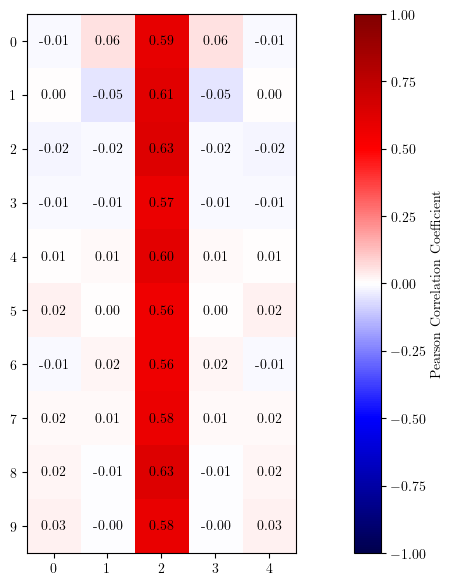
\includegraphics[width = 0.5\textwidth]{Figures/logits_correlation.png}
	\caption{Pearson $r^2$ value for each logit in the ouput of the transition model between $g(s, a)$ and $\ell_r^\mathcal{S}g(\ell_r^\mathcal{S}s,\ell_r^\mathcal{A}a)$, for one of the 675 possible sate action pairs, across 1000 random  seeds for network initialization. }
	\label{fig:logits_correlation}
\end{figure}
Empirically one can see the lack of correlation in Fig.\ref{fig:logits_correlation}, which plots the $r^2$ co-efficient between the transition images across 1000 randomly initialized untrained networks. The network parameterise the next states as two distributions, by outputing an array of 50 logits. As expected, the network responses along the center axis should be invariant to the input transformation. Thus, a positive correlation co-efficient is encouraging. For all other logits in the distribution over the next state there is no evidence of a correlation between the two transition images, at a 5\% significance level.

With the two ouptut's being independent of each other, then correct next state can be selected using the proximal layer reliably, and the networks can be approximately equivariant.



\subsection{CartPole}
A CartPole transition model is a functional approximation to a deterministic Non linear system. In CartPole the transitions between different states in CartPole are governed by the PDEs:
\begin{equation}
	\ddot{\theta} = \frac{g \sin \theta + \cos\theta \left({\frac{-F - m_p l \dot{\theta}^2 \sin(\theta)}{m_c + m_p}} \right )}{l\left ( \frac{4}{3} - \frac{m_p \cos^2 \theta}{m_c + m_p}\right)},
\end{equation}

\begin{equation}
	\ddot{x} = \frac{ F + m_p l (\dot{\theta}^2 \sin \theta - \ddot{\theta} \cos \theta)}{m_c + m_p}.
\end{equation}
Here $g$ is the acceleration due to gravity and is positive, $\theta$ is the angle between the pole and vertical, with the pole length $l$. $F$ is the action force, where the positive direction is right. The masses of the cart and the pole are $m_c, m_p$, respectively. Finally $\dot{}$, indicates a derivative with respect to time.

These PDEs have no closed solution and their form is taken from \cite{florian2007correct} who provides slight corrections to the original dynamics in \cite{barto1983neuronlike}.

To learn this transition model, transitions are sampled from a policy on the MDP, and stored. This is then used as a dataset to perform supervised learning on. The Transition model, $T_\phi: \mathcal{S} \times \mathcal{A} \rightarrow \mathcal{S}$, predicts next states from a state action pair. A state is a vector s:
\begin{equation}
	s = \begin{pmatrix}
		x       \\
		\dot{x} \\
		\theta  \\
		\dot{\theta}
	\end{pmatrix}
\end{equation}
The loss function for the transition model is the average L2 distance between the predicted next state, and the true next state across a batch of samples.
\begin{equation}
	L(\phi) = \frac{1}{N}\sum^N_{(s, a, s')_i \sim \mathcal \tau} ||T(s, a) - s'||_2
\end{equation}
Here $\tau = \{(s, a , s')_1^N\}$ is a batch of transition, of size $N$, sampled from the MDP, and $(s, a, s')$, is the state, action, next state tuple. Often a reward model is required to also make an MDP. For simplicity, the CartPole reward model is used, rather than learned. As such the transition gains a reward of $+1$, if $|\theta| < 12.5^o$, otherwise the episode terminates.

\subsubsection{Constructing Equivariant World Models}
Like in the previous section on \ref{sec:actor-critic}, the equivariant transition models are deep G-CNNs. In contrast to equivariant Actors in the previous section, these networks have to use the proximal pooling layer on their output \ref{sec:proximal_pool}. The equivariance described by these nextworks is to the identity and negative operation, such that;
\begin{equation}
	T(- s, 2*a - 1) =  -T(s, a), \forall
\end{equation}
These transition models, are not truely equivariant but empirically the proximal pooling layer suffices to meet the equivariance condition.

Again in a similar fashion to the actor networks, the transition models have two hidden Group Covolution layers. The input layer for actions also transforms the action from $[0, 1]$ to $[-1, 1]$. Thus the same group convolution layer can be used for both the state and the action input.

\subsubsection{Comparing Convergence of Transition Models}
In order to perform model based RL a transition model must be learnt to simulate transitions, such that the agent can learn a policy that performs better in the original environment. Thus the first set of experiments were training transition models in a supervised learning setting.

Three different pairs of models were trained. The first pair on data collected from an expert and random policy. The second pair took the first dataset and filtered out the transitions which took the right action. The final pair is trained only on data sampled from a random policy.
\begin{figure}
	\centering
	\includegraphics*[width=\linewidth]{Figures/transition_model_cp.png}
	\caption{Transition Model RMS error, plotted against epochs for three different training datasets. Left, the dataset contains a 50/50 split between expert policy sampled transitions, and transitions sampled from a random policy with 80,000 transitions. Center, the same dataset as left, however, with only the left action taken. This dataset contains 40,000 transitions. Right, solely transitions sampled from a random policy, again with 80,000 transitions. All plots have the same set of validation data with a 50/50 split of expert and radom policy sampled data.}
	\label{fig:transition_model_cp}
\end{figure}
In Fig.\ref{fig:cartpole_equivariant_actor} it is clear that the G-CNN despite having the same parameter count, performs substantially better on all 3 datasets. Further, there is a reassuringly stark delta in performance between the equivariant model, and the conventional MLP transition model, when the right action is filtered out. The equivariant model recovers the majority of the performance in this scenario, while the MLP appears to ...

% TODO

\subsection{Catch}
In catch the transitions between states are much simpler with the updates to the ball position between timesteps.
\begin{equation}
	y_{t+1} = y_t + 1.
\end{equation}
And the paddle displacement is goverend by,
\begin{equation}
	x_{t+1} = \text{clip}(1- a_t + x_t, 0, 5).
\end{equation}
Above the clip fucntion, stops the paddle moving beyond the environment's boundaries. The observations from the environment are arrays of shape $5 , 10$, with two ones, indicating the ball and paddle position. The paddle is in row 9, and the ball is only allowed in rows $0 -8$. To encode these constraints the network parameterises two distributions over the ball and paddle locations. The ball can be in one of 45 states, and the paddle may be in one of 5 states. The outputs of the networks are then the logits of the two distributions. In order to predict the next state, the mode of the distributions is taken for both the ball and the paddle. 

Again construction of the G-CNN is much the same as in the case for CartPole, the basic network built from group convolutions. Again two hidden layers are used. Typically for a network predicting distributions against logits, the Binary Cross Entropy loss is used, however, it was found that this was not as effective as using the L2 distance between the logits, and the observation. Thus the loss function to train both transition models was,
\begin{equation}
	L(\phi) = \frac{1}{N}\sum_{(s, a, s') \sim \tau}^N (1 - \delta(\text{done}))||T(s, a) - s'||_2 \end{equation} Here, the one subtlety is that the loss is only back propagated if $s$, is not a terminal state. The indicator function $\delta(\text{done}) = 1 \text{if $s$ is terminal} $. Thus the model only learns transitions goverend by the environment dynamics, and not how to reset the episode.

In order to make the model equivariant the proximal pooling layer a distance metric needs to be used that quantifies how far apart the predictions are. The metric used is an L1 loss between the x, y position in s and s' of both the ball and the paddle. Additionally, to make the possible number of distances greater when the distances are summed, the ball's displacement is multiplied by 0.13. This constant value was found to improve the equivariance behaviour of the proximal pooling layer. The distance metric is then given by,
\begin{equation}
	d(s, s') = ||\text{mode}(T(s, a)_b) - s'_b||_1 + 0.13 ||\text{mode}T(s, a)_p - s'_p||_1.
\end{equation}
The subscripts, $b, p$ indicate the ball and the paddle distributions respectively.

\subsubsection{Comparing Convergence of Transition Models}
In the same manner as before for CartPole, the transition models were trained on three different datasets to asses their convergence behaviour. In the same vein these were a random and expert policy sampled data, only left actions from the previous dataset, and only random policy sampled transitions. 

\begin{figure}
	\centering
	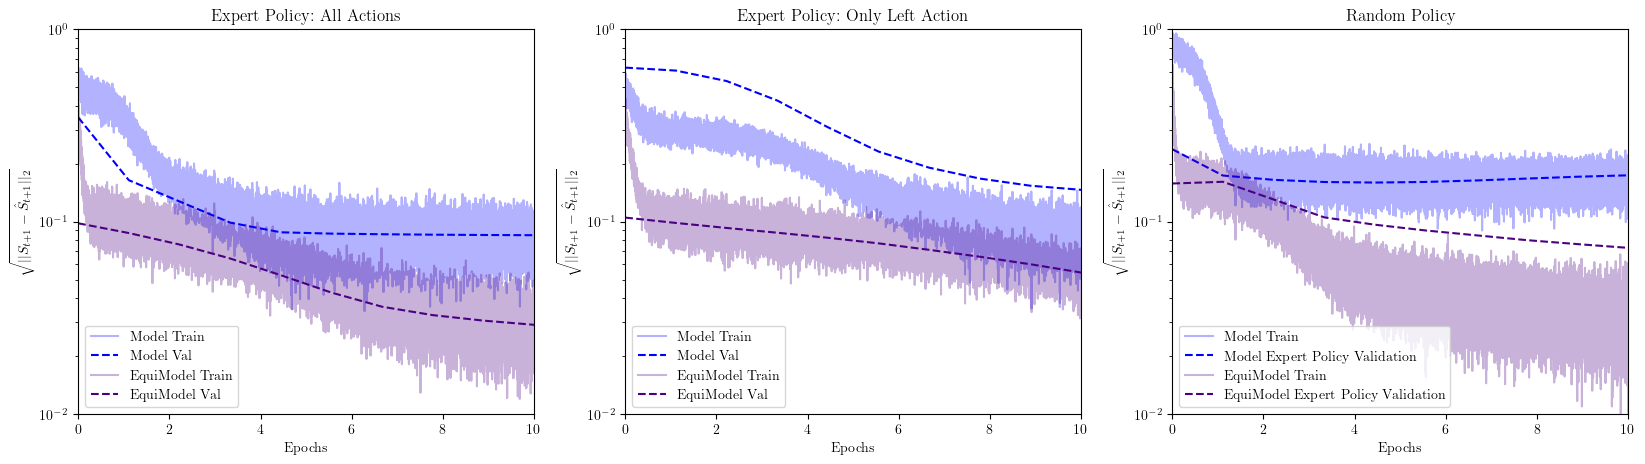
\includegraphics[width=\linewidth]{Figures/transition_model_cp.png}
	\label{fig:transition_model_catch}
	\caption{something}
\end{figure}

\ldots
% TODO: Descriptions and something.




% \chapter{My First Content Chapter}
\label{chapterlabel2}

% This just dumps some pseudolatin in so you can see some text in place.
\blindtext

% \section{Notes}

\textbf{Definition: MDP Homomorphism} Given some MDP $\mathcal{M}$, where there
exists a surjective map, from $\mathcal{S} \times \mathcal{A} \rightarrow \omc{S} \times
	\omc{A}$. the MDP $\omc{M}$ is an abstract MDP over the new space. The
homomorphism $h$, then is the tuple of $(\sigma, \alpha_s|s \in \mathcal{S})$, where
$\sigma: \mathcal{S} \rightarrow \omc{S}$ and $\alpha_s : \mathcal{A} \rightarrow \omc{A}$.
This surjective map must satisfy two constraints for it to be a valid MDP
homomorphism; \begin{enumerate} \item $R(s, a) = R(\sigma(s), \alpha_s(a))$
	\item $T(s', a, s) = T(\sigma(s'), \alpha_s(a), \sigma(s))$ \end{enumerate}


Rather than learning a tranditional MDP homomorphism, we wish to learn a homomorphic map

$$h: \mathcal{A} \times \mathcal{S} \times \overline{\mathcal{A}} -> \omc{S}$$

With the constraints that the homomorphsim in the simplest case maps of invertersion symmetry $D_2$ where in state space the $D_2$ representtion is $L_2$ and in action space the $D_2$ representaiton is $K_2$. so that $$h(a, s, \overline{a}) = h(K_2 a, L_2 s, \overline{a})$$.

Because we are learning from determinsistic dynamics $T: \mathcal{S} \times \mathcal{A} \rightarrow \mathcal{S}$ and $\overline{T}: \omc{S} \times \omc{A} \rightarrow \omc{S}$ we must also learn that

$$\overline{T}(\overline{s}, \overline{a}) = h(T(s, a), a', \overline{a})$$.

where $overline{s} = h(s, a, \overline{a})$

$$\overline{T}(h(s, a, \overline{a}), \overline{a}) = h(T(s, a), a', \overline{a})$$.


In the case of the cartpole the actions $a, \overline{a} \in [0, 1]$.


\subsection{Training}
The objectiive of training is to use some kind of similarity metric like that used in Approximate MDP Homomorphisms to learn the parametric form of $h$ in a supervised setting, over these (state, action, abstract action, next state) tuples.
With the hypothesis that having a group equivariant network will make the learning more efficient.

% \chapter{General Conclusions}
\label{chapterlabel4}

% This just dumps some pseudolatin in so you can see some text in place.
\blindtext

% \addcontentsline{toc}{chapter}{Appendices}

% The \appendix command resets the chapter counter, and changes the chapter numbering scheme to capital letters.
%\chapter{Appendices}
\appendix
\chapter{An Appendix About Stuff}
\label{appendixlabel1}
(stuff)

\chapter{Another Appendix About Things}
\label{appendixlabel2}
(things)

\chapter{Colophon}
\label{appendixlabel3}
\textit{This is a description of the tools you used to make your thesis. It helps people make future documents, reminds you, and looks good.}

\textit{(example)} This document was set in the Times Roman typeface using \LaTeX\ and Bib\TeX , composed with a text editor. 
 % description of document, e.g. type faces, TeX used, TeXmaker, packages and things used for figures. Like a computational details section.
% e.g. http://tex.stackexchange.com/questions/63468/what-is-best-way-to-mention-that-a-document-has-been-typeset-with-tex#63503

% Side note:
%http://tex.stackexchange.com/questions/1319/showcase-of-beautiful-typography-done-in-tex-friends

% You could separate these out into different files if you have
%  particularly large appendices.

% This line manually adds the Bibliography to the table of contents.
% The fact that \include is the last thing before this ensures that it
% is on a clear page, and adding it like this means that it doesn't
% get a chapter or appendix number.
\addcontentsline{toc}{chapter}{Bibliography}
% Actually generates your bibliography.

\bibliography{bibliography}
% All done. \o/
\end{document}
